\chapter{Multiplexed Sequences} \label{appendices::AppendixA}

Multiplexed Sequences are currently used to model data access from multi channel 
ADC's. Samples over all n ADC channels, taken at the same point in time $T_0$ 
are 
placed consecutively in memory. The next set of samples taken at $T_1$ for the n 
ADC channels follow the previous data in memory and so on (see Figure 
\ref{mux_data}). Such 
an area in memory which contain data in this described order is represented by 
the \texttt{AREA\_MULTIPLEXED\_SEQUENCE\_<area\_name>} keyword. Each ADC channel 
is described by the \\
\texttt{SEQUENCE\_<area\_name>\_<sequence\_number>} keyword.


\begin{figure}[htbp] 
    \centering
    \includegraphics[width=.5\textwidth]{images/MuxedSequences.pdf} \caption{The
    Multiplexed Data Region Representation} \label{mux_data} \end{figure}


Such Multiplexed data regions are described in the map files as below :

{\ttfamily  
\begin{lstlisting} 
BOARD.AREA_MULTIPLEXED_SEQUENCE_DMA 0x0 0x0 0x100  0x2
BOARD.SEQUENCE_DMA_0 0x1 0x00 0x4 0x2 32 0 1
BOARD.SEQUENCE_DMA_1 0x1 0x04 0x4 0x2 16 0 0
BOARD.SEQUENCE_DMA_2 0x1 0x06 0x4 0x2 16 0 0
\end{lstlisting} 
}

The \texttt{BOARD} prefix denotes that, the described resource belongs to the 
module `BOARD'.The \texttt{AREA\_MULTIPLEXED\_SEQUENCE\_DMA} keyword describes 
the span of the multiplexed region to be $\mathtt{0x100}$ bytes. The subsequent 
3 lines 
describes the data on the 3 channels that have been multiplexed to this region. 
\texttt{SEQUENCE\_DMA\_0} describes that each sample of this channel takes up 
$\mathtt{0x4}$ bytes, and has a Fixed point representation spanning 32 bits with 
0 fractional and one sign bit. \texttt{SEQUENCE\_DMA\_1} describes that a 
sampled data on the second channel takes up $\mathtt{0x4}$ bytes and has a Fixed 
point representation spanning 16 bits with 0 fractinal bits and no sign bit. The 
interpretation is similar for the 3$^{rd}$ channel.

Figure \ref{mux_qthardmon} shows \texttt{BOARD.AREA\_MULTIPLEXED\_SEQUENCE\_DMA} 
in QtHardMon. Clicking on \texttt{SEQUENCE\_DMA\_X} demultiplexes the data from 
the \\
\texttt{AREA\_MULTIPLEXED\_SEQUENCE\_DMA} region and displays all elements 
belonging to the selected Sequence/(ADC channel) in the Register Values 
table. These values may be modified and written back to the \\
\texttt{BOARD.AREA\_MULTIPLEXED\_SEQUENCE\_DMA} region. QtHardmon ensures that 
the data would be multiplexed and put into the correct position within the area 
on clicking the write button.

\begin{figure}[htbp] 
    \centering
    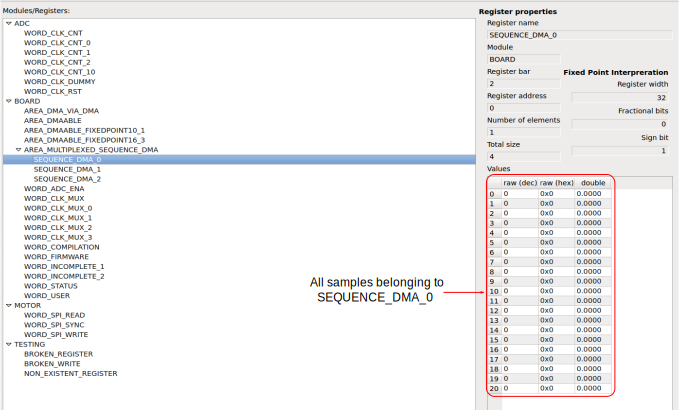
\includegraphics[width=1\textwidth]{images/MuxAccessorInQtHardMon.pdf} 
\caption{Multiplexed Region in QtHardMon} \label{mux_qthardmon} \end{figure}




